\documentclass[11pt]{exam}

\usepackage{amsmath}
\usepackage{graphicx}
\usepackage{geometry}
\usepackage{etoolbox}
\BeforeBeginEnvironment{choices}{\par\nopagebreak\minipage{\linewidth}}
\AfterEndEnvironment{choices}{\endminipage}
\geometry{
a4paper,
total={185mm,257mm},
left=10mm,
top=25mm,
bottom=10mm
}

\begin{document}
\setlength{\voffset}{-0.5in}
\setlength{\headsep}{5pt}

\fbox{\fbox{\parbox{8cm}{\centering
\vspace{2mm}
Testat - Versuch E - Diffusion und Osmose 
\vspace{2mm}
}}}
\hspace{2mm}
\makebox[0.25\textwidth]{Name:\enspace\hrulefill} \hspace{5mm}
\makebox[0.2\textwidth]{Datum:\enspace\hrulefill}
\vspace{4mm}

\begin{questions}

\question Die Leitfähigkeit von 30 ml Salzlösung wird zu 5,0 \( \frac{\mu S}{cm} \) bestimmt. Welches Volumen an destilliertem Wasser muss zugeführt werden, um eine Leitfähigkeit von 3,0 \( \frac{\mu S}{cm} \) zu messen?

\begin{choices}
	\choice 20 ml
	\choice 0 ml
	\choice 30 ml
	\choice 40 ml
	\choice 60 ml
\end{choices}

\vspace{3mm}\question In folgender Abbildung sehen Sie zwei Kammern, die durch eine semipermeable Membran getrennt sind. In der linken Kammer befindet sich zu Beginn eine Zuckerlösung, in der rechten nur Wasser. Das Wasser kann die Membran ungehindert durchdringen, der Zucker nicht. Welche Abbildung zeigt den Gleichgewichtszustand, der sich nach einiger Zeit einstellt? 

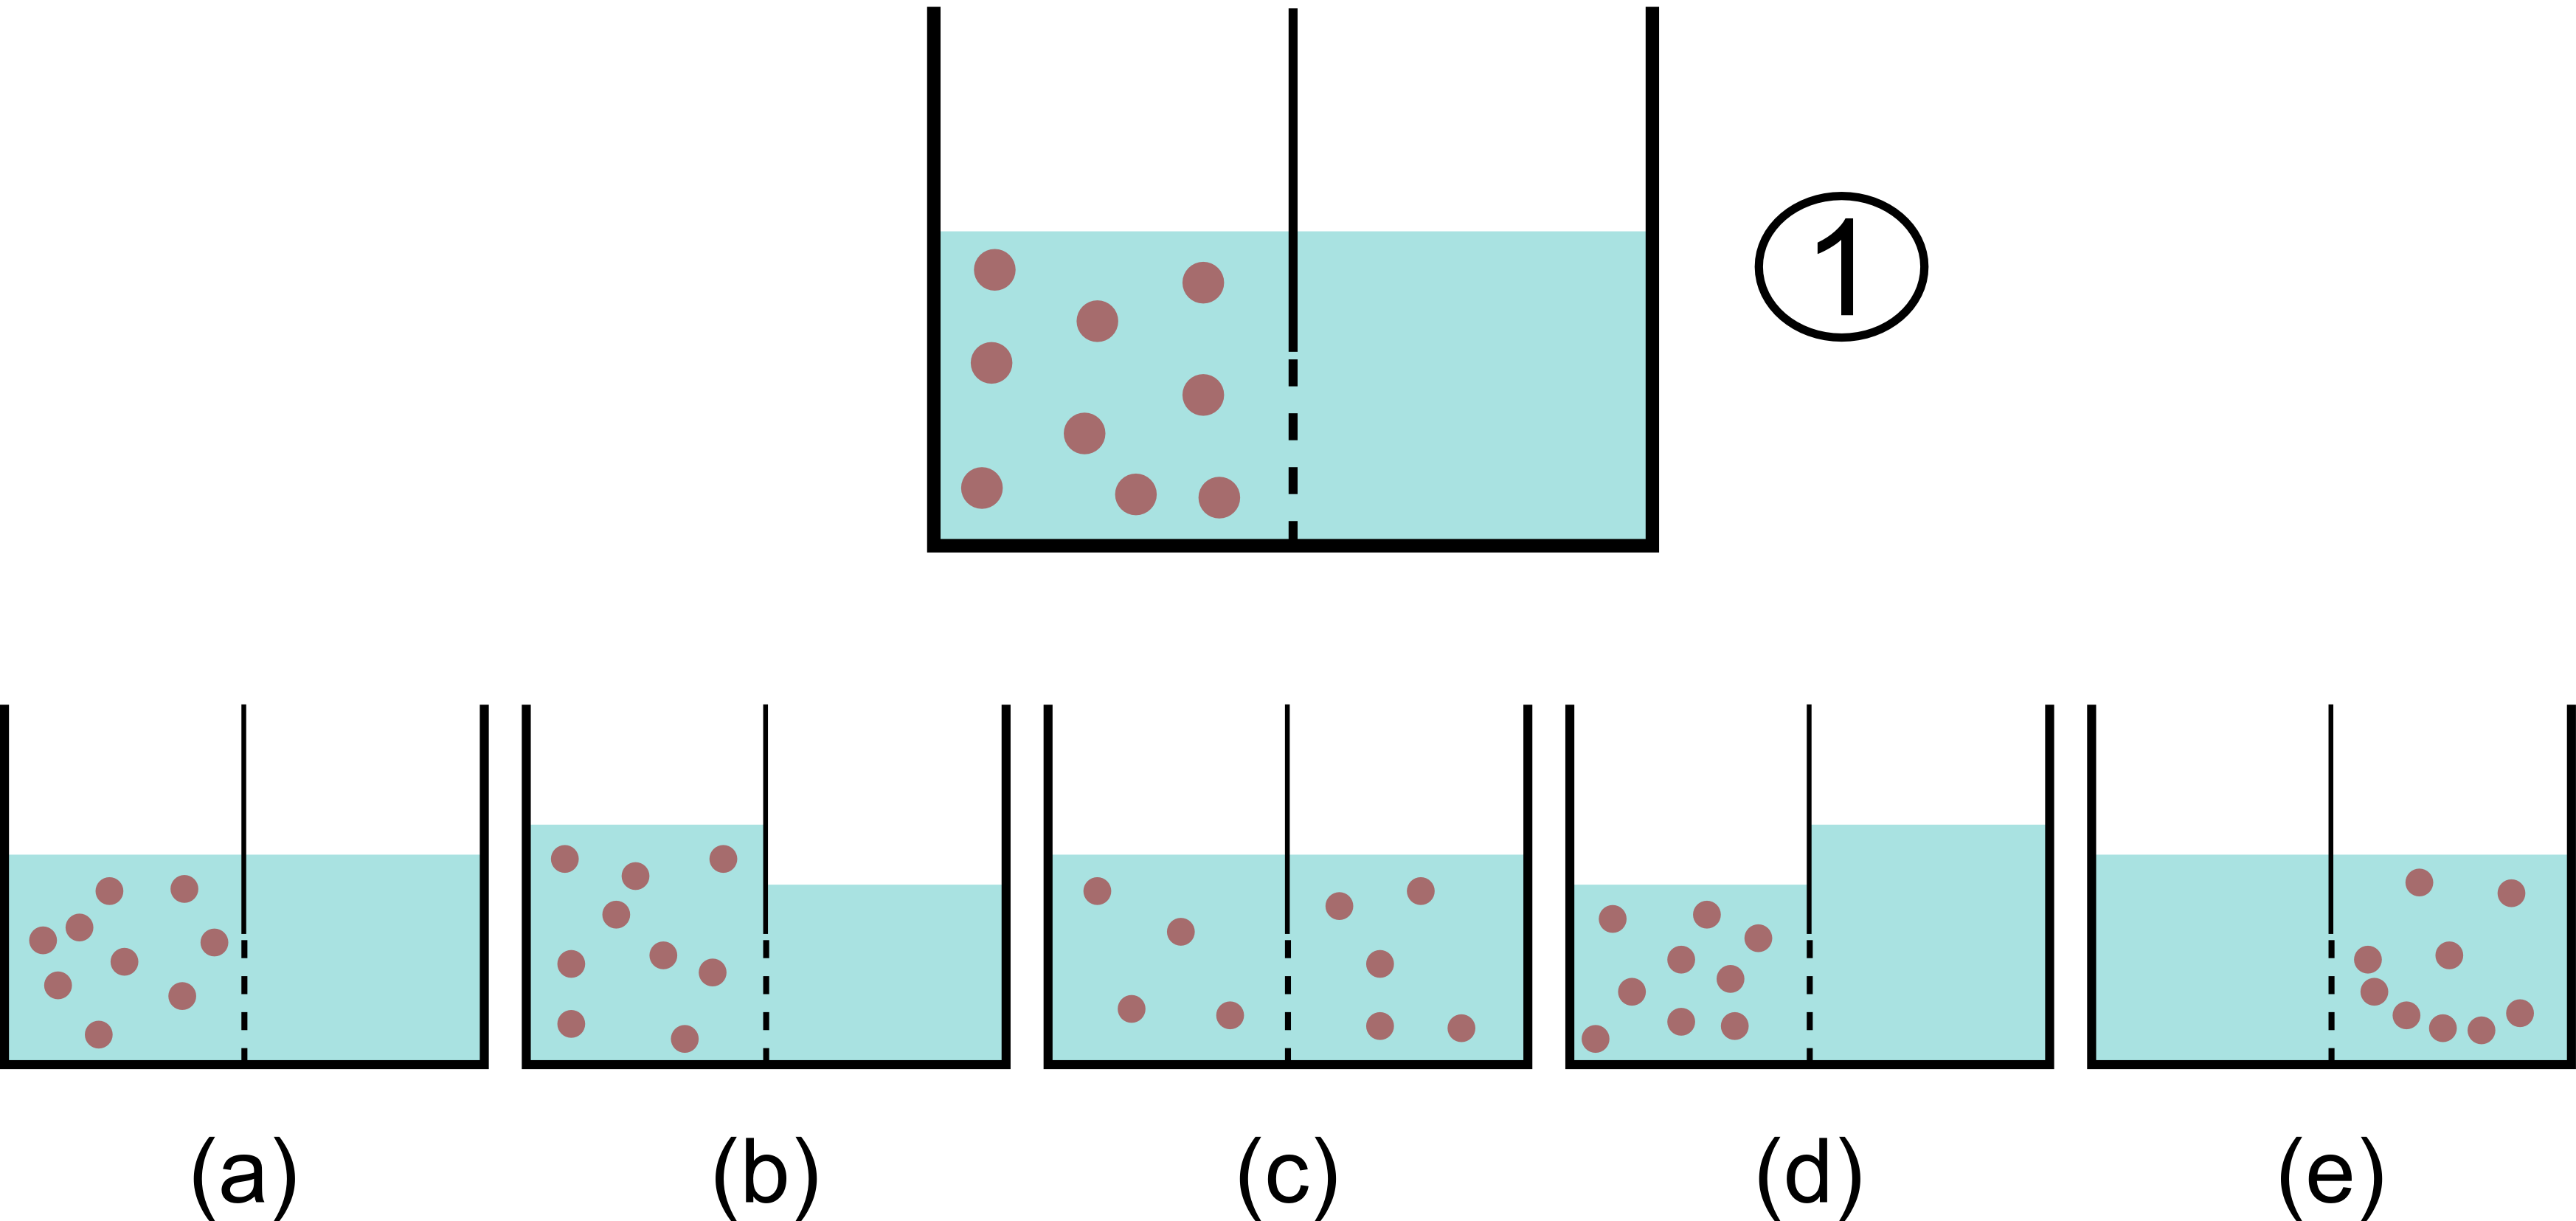
\includegraphics[width=0.4\textwidth]{images/Osmose.png}

\begin{choices}
	\choice a)
	\choice c)
	\choice b)
	\choice e)
	\choice d)
\end{choices}

\vspace{3mm}\question Der Diffusionsfluss durch eine rechteckige Membran mit den Seitenlängen 25 mm und 1 cm ist 1,5 \(\frac{mg}{s} \). Wie groß ist der Diffusionsfluss, wenn stattdessen eine Membran mit den Seitenlängen 5 cm und 10 mm verwendet wird?

\begin{choices}
	\choice \( J = 2,5 \frac{mg}{s} \)
	\choice \( J = 3,5 \frac{mg}{s} \)
	\choice \( J = 2,0 \frac{mg}{s} \)
	\choice \( J = 3,0 \frac{mg}{s} \)
	\choice \( J = 1,5 \frac{mg}{s} \)
\end{choices}

\vspace{3mm}\question Wo spielt Diffusion in der Natur keine Rolle?

\begin{choices}
	\choice Gasaustausch bei der Lungenatmung
	\choice Bildung des Zellpotentials
	\choice Filtration in der Niere
	\choice Bildung von Ödemen
	\choice Bewegung von Amöben
\end{choices}

\vspace{3mm}\question Die Angabe des Diffusionskoeffizienten \( D={6,0 \cdot 10^{-9}} \frac{m^2}{s} \) ist äquivalent zu

\begin{choices}
	\choice \( D={0,36 \cdot 10^{-3}} \frac{mm^2}{min} \)
	\choice \( D={1,0 \cdot 10^{-6}} \frac{mm^2}{min} \)
	\choice \( D={0,1 \cdot 10^{-2}} \frac{mm^2}{min} \)
	\choice \( D={36 \cdot 10^{2}} \frac{mm^2}{min} \)
	\choice \( D={3,6 \cdot 10^{-1}} \frac{mm^2}{min} \)
\end{choices}

\vspace{3mm}\end{questions}

\end{document}
